% -*- mode : latex; coding: utf-8 -*-
\chapter{Evaluation} \label{sec:evaluation}

\section{Experimental Setup} \label{sec:exp-setup}

I evaluate the performance of CXL type 3 device using \textit{CXLmem} simulator. In this evaluation, I focused on the impact of CXL type 3 device to overall system performance. I compared the performance of CXL type 3 device to the performance of local DRAM memory. I controlled page allocation ratio between CXL type 3 device and local DRAM memory. If all the pages are allocated to local DRAM memory, all the memory requests will be sent to local DRAM memory. I call this case as ``DIMM''. On the contrary, if all the pages are allocated to CXL type 3 device, all the memory requests will be sent to CXL type 3 device. I call this case as ``MXP'' which means memory expander. Also, I allocated pages on both local DRAM and CXL type 3 device with fixed ratio. In this case, I call ``MIX''.

\subsection{Simulator Setup}
\label{sec:simulator-setup}
CXLmem can run as a standalone simulator with memory trace. However, in this research, to evaluate the overall performance of system and to estimate the impact of CXL type 3 device on the system, I attach CXLmem to MacSim \cite{MACSIM}, a Pin-based cycle-level x86 simulator.

CXL type 3 device is basically memory device. Therefore, it's necessary to attach memory simulator to CXLmem. I use Ramulator \cite{RAMULATOR}, a trace-driven and cycle-accurate DRAM simulator. For the fair comparison between CXL type 3 device and local DRAM memory, I also use Ramulator as a local DRAM memory of MacSim.

Table \ref{tab:configuration} shows the configuration of CPU, DRAM, CXL in this research.

\begin{table}[t]
  \centering
  \caption{CPU, DRAM, CXL Configuration in this research}
  \label{tab:configuration}
 \begin{tabular}{|c || c|} 
 \hline
 \multicolumn{2}{|c|}{\textbf{CPU}} \\
 \hline
 Core & 4 cores, 4.0GHz, out-of-order \\ 
 L1 cache & 8-way 32KB I-Cache (1-cycle), 16-way 48KB D-Cache (3-cycle) \\
 L2 cache & 16-way 2MB private (8-cycle) \\
 L3 cache & 32-way 8MB (4-slice, 30-cycle) \\
 \hline \hline
 \multicolumn{2}{|c|}{\textbf{DRAM (Both local DRAM and CXL type 3 device)}} \\
 \hline
 Bus frequency & 1.2GHz (DDR 2.4GHz), 8B per channel \\
 Channel/Rank & 1/2 \\
 \hline \hline
 \multicolumn{2}{|c|}{\textbf{CXL interconnect}} \\
 \hline
 Bus frequency & 1.6GHz \\
 Virtual Channel Buffer & One channel for each message type, 32 entries \\
 Latency & Transaction (5, 10, 20-cycle), Data Link (5, 10, 20-cycle) \\
 Bandwidth & 32GT/s per lane, 16 lanes, 64 GB/s per direction \\
 \hline
 \end{tabular}
\end{table}



\subsection{Workload Setup}
\label{sec:workload-setup}
I use SPEC CPU2006 benchmarks. To see the impact of CXL type 3 device on overall system performance, I selected memory-intensive workloads from SPEC CPU2006. I ran 100M instructions on MacSim configured as single core, LLC 512 KB. I selected 4 workloads that show high LLC MPKI (Miss Per Kilo Instructions). High LLC MPKI means more requests are sent to memory device, which implies memory-intensive workload. Those selected memory-intensive workloads are mcf, leslie3d, bwaves, soplex. mcf is an application that is related to combinatorial optimization. leslie3d and bwaves are related to fluid dynamics. soplex is related to linear programming and optimization. I set up 8 workload mixes using 4 memory-intensive workloads. Since all the workloads are single-threaded and I simulated with 4 cores, all the workload mixes contains 4 workloads. Table \ref{tab:workload-setup} shows 8 workload mixes and LLC MPKIs. All the LLC MPKI values are about single workload. Thus, for workload mixes that two or more workloads are mixed, LLC MPKI is shown as N/A.
For each workload, I simulated 500M cycles of execution.

\begin{table}[t]
  \centering
  \caption{Evaluated Workloads}
  \label{tab:workload-setup}
 \begin{tabular}{|c | c | c|} 
 \hline
 \textbf{Mix} & \textbf{Workloads} & \textbf{LLC MPKI (single)} \\
 \hline
 WL-1 & 4 x mcf & 118.61 \\
 \hline
 WL-2 & 4 x leslie3d & 45.07 \\
 \hline
 WL-3 & 4 x soplex & 44.80 \\
 \hline
 WL-4 & 4 x bwaves & 66.02 \\
 \hline
 WL-5 & mcf-leslie3d-soplex-bwaves & N/A \\
 \hline
 WL-6 & mcf-mcf-leslie3d-leslie3d & N/A \\
 \hline
 WL-7 & soplex-soplex-bwaves-bwaves & N/A \\
 \hline
 WL-8 & mcf-mcf-bwaves-bwaves & N/A \\
 \hline
 \end{tabular}
\end{table}


\section{Evaluation Result}
\label{sec:evaluation-result}


\subsection{Overall Performance}
\label{sec:overall-performance}
Figure \ref{fig:ipc} shows normalized IPC (instruction per cycle) of diverse configurations for 8 workloads. The baseline is DIMM, when all the requests sent to local DRAM. 3:1, 2:2, 1:3 shows the page allocation ratio between local DRAM and CXL type 3 device. In case of 3:1, 3/4 of all the pages are allocated to local DRAM and the leftover pages are allocated to CXL type 3 device. MXP shows the performance when all the memory request are sent to CXL type 3 device.

\begin{figure}[ht]
  \centering
  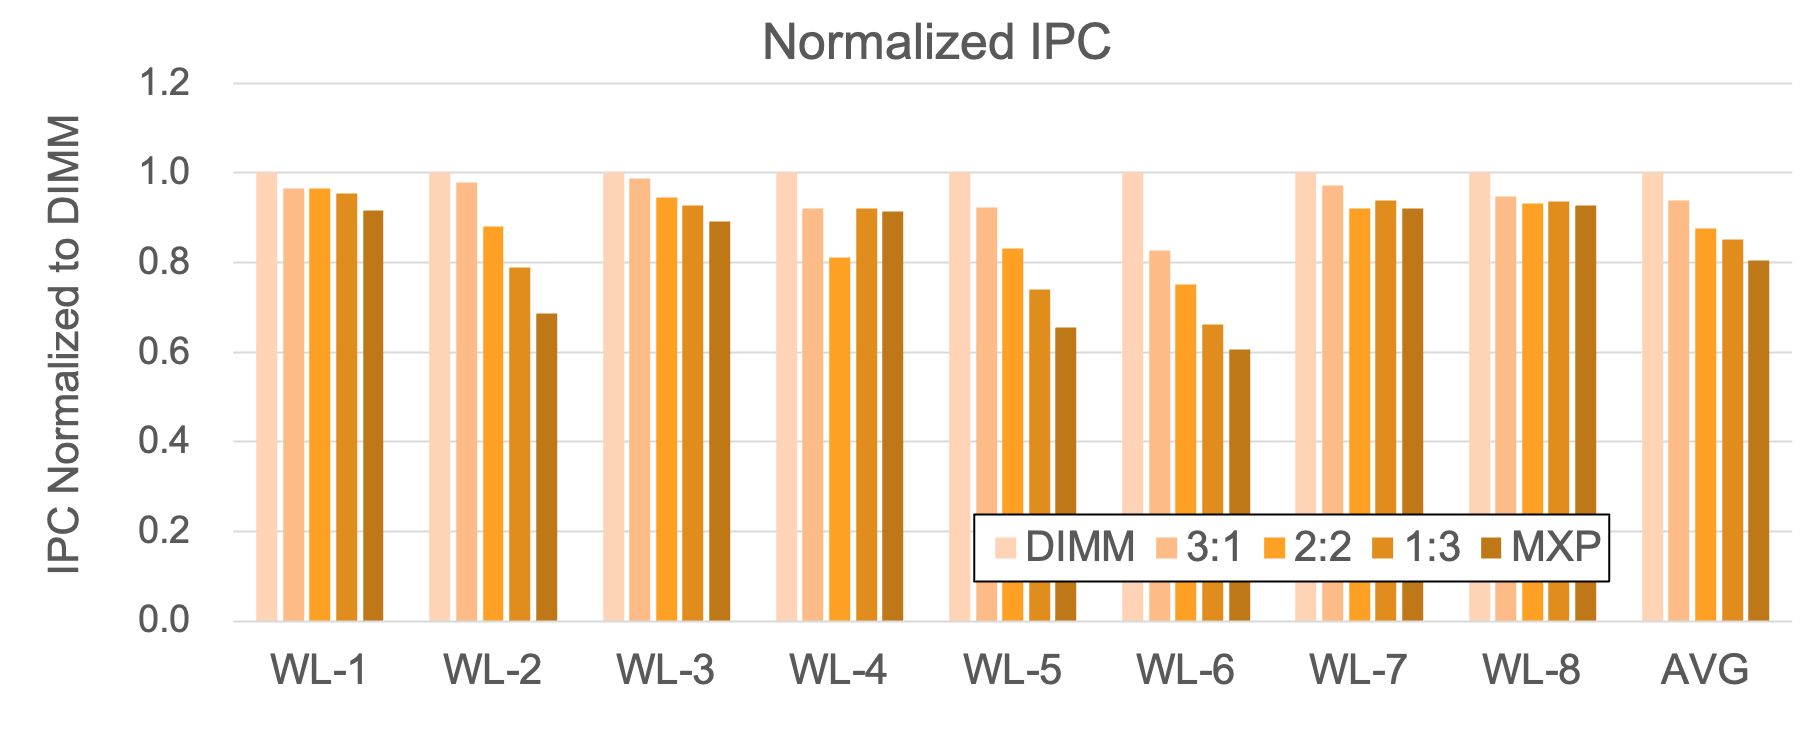
\includegraphics[width=\textwidth]{figures/ipc.png}
  \caption{IPC normalized to DIMM. As pages allocated to CXL type 3 device increase, IPC drops.}
  \label{fig:ipc}
\end{figure}

On average, MXP achieves 0.8 normalized IPC in Figure \ref{fig:ipc}. This result comes from CXL interconnection's overhead. While DIMM just sends memory request to DRAM, MXP should go through all three layers in master and slave. Performance degradation fluctuates a lot as workload changes. This comes from each workloads memory access characteristics. Regardless of workload, MXP always experience performance degradation. Also, as memory requests to CXL type 3 device increase, the IPC dropped. On average, 3:1's normalized IPC is 0.94, 2:2's normalized IPC is 0.88, 1:3's normalized IPC is 0.85. As memory requests toward CXL type 3 device increase, the impact of CXL interconnection gets larger naturally. These results imply that although CXL type 3 device can provide larger capacity, always there exist performance degradation. When considering CXL type 3 device as a memory expander, we also need to consider the impact on overall system performance. On Figure \ref{fig:ipc}, 2:2 on WL-4 shows weird large performance degradation. That might be caused by gap between page allocation ratio and memory request ratio. Although I allocated pages with 2:2 ratio, the memory request ratio might not be always equal. Thus there might be some unexpected result.


\subsection{Read Latency}
\label{sec:Read Latency}
This evaluation result focuses on read latency. While instruction with read request can't do anything until response comes, instruction with write request can proceed after sending request. Thus read latency has greater impact on overall performance. So, I focused on read latency. Figure \ref{fig:rd-latency} shows read latency of DIMM and MXP for 8 workloads. The metric of read latency is CPU cycle.

\begin{figure}[ht]
  \centering
  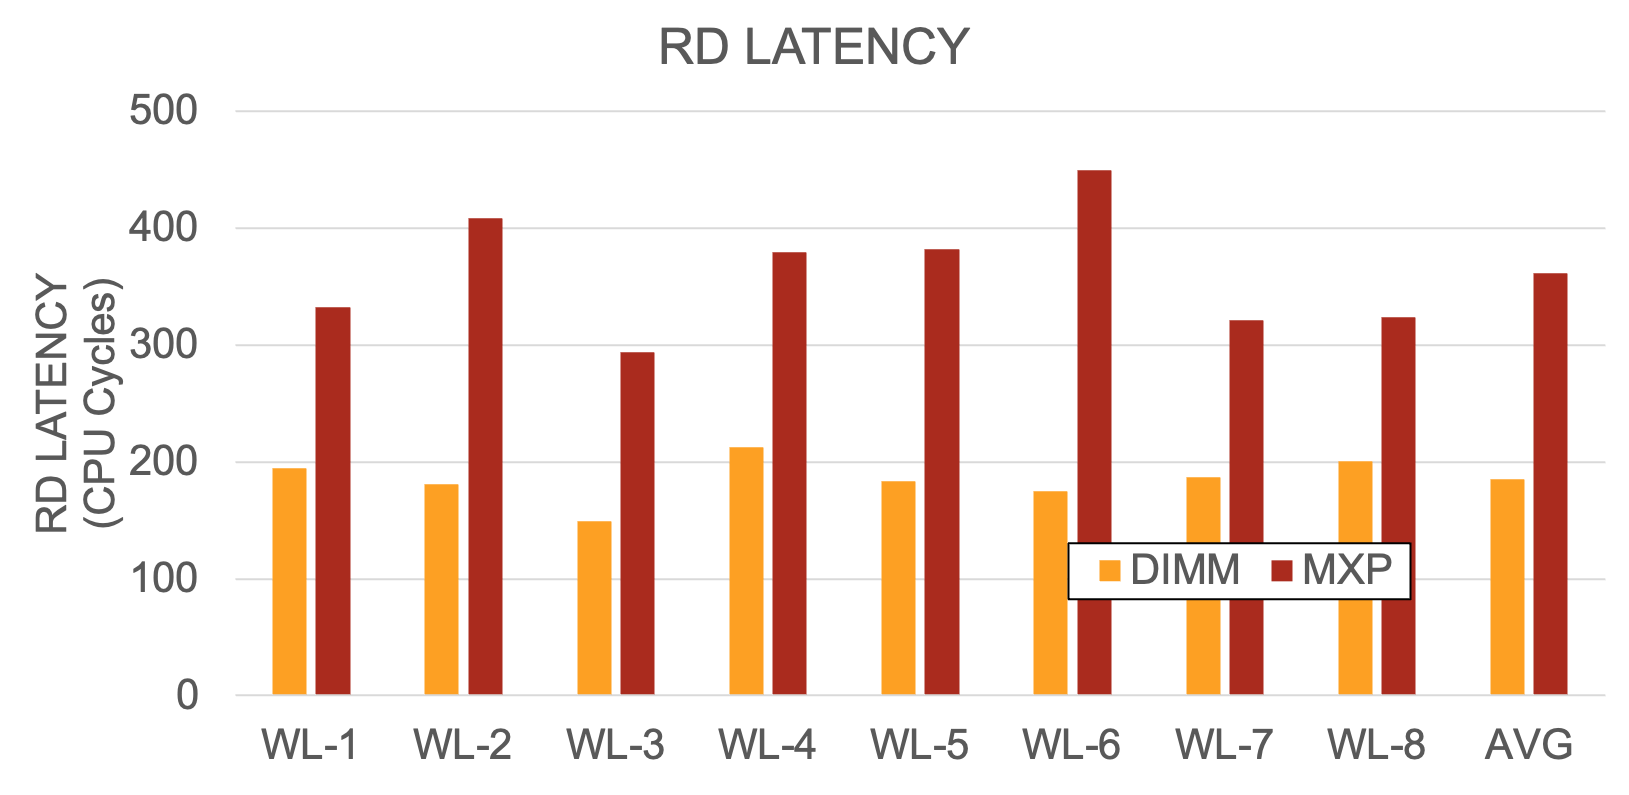
\includegraphics[width=\textwidth]{figures/rd latency.png}
  \caption{Read latency comparison between DIMM and MXP. On average, MXP's read latency is nearly double of DIMM's read latency.}
  \label{fig:rd-latency}
\end{figure}

On average, MXP's read latency is almost double of DIMM's read latency in Figure \ref{fig:rd-latency}. MXP's average read latency is 361.35 cycles, while DIMM's average read latency is 185.43. Since DIMM is local DRAM memory, the read latency only includes memory access latency. However, MXP includes not only memory access latency, but also CXL transaction latency. CXL transaction latency is not always static, because flit packing not always serves first come request first. Although some request has arrived earlier, if it doesn't satisfy flit packing policy or there exist other type of requests that satisfy flit packing policy or slave doesn't have enough free space to receive that request, the transaction of request might be delayed and the request should wait more cycles in virtual channel buffer. Thus, CXL transaction latency is not simply sum of each layer's static latency, but includes some dynamic latency. However, in general, CXL type 3 device shows nearly double latency than local DRAM memory. This result implies two crucial points to consider. First, if we only use CXL type 3 device, memory access latency gets doubled. Thus, memory latency bound workloads may get serious performance degradation. So we should not use only CXL type 3 device as main memory. Instead, we should use both local DRAM and CXL type 3 device. Second, although we use both local DRAM and CXL type 3 device, still CXL type 3 device's long latency may have bad influence on system. If we access CXL type 3 device too often, the impact might be larger. Thus, we should consider how to locate frequently accessed data in local DRAM memory and cold data in CXL type 3 device.

Figure \ref{fig:avg-rd-latency} shows CXL type 3 device read latency of MIX and MXP with diverse configuration. X-axis names show the configuration. There are 3 fields in each name. The first represents mode, MXP or MIX. In case of MIX, page allocation ratio between CXL type 3 device and local DRAM is 1:1. The second and third field shows transaction layer latency, data link layer latency in CPU cycle. The value of each configuration is average of 8 workloads CXL type 3 device read latency. The left most bar shows the local DRAM read latency in DIMM. This bar is inserted to easily understand scale of MXP, MIX latency. The metric of read latency is CPU cycle.

\begin{figure}[ht]
  \centering
  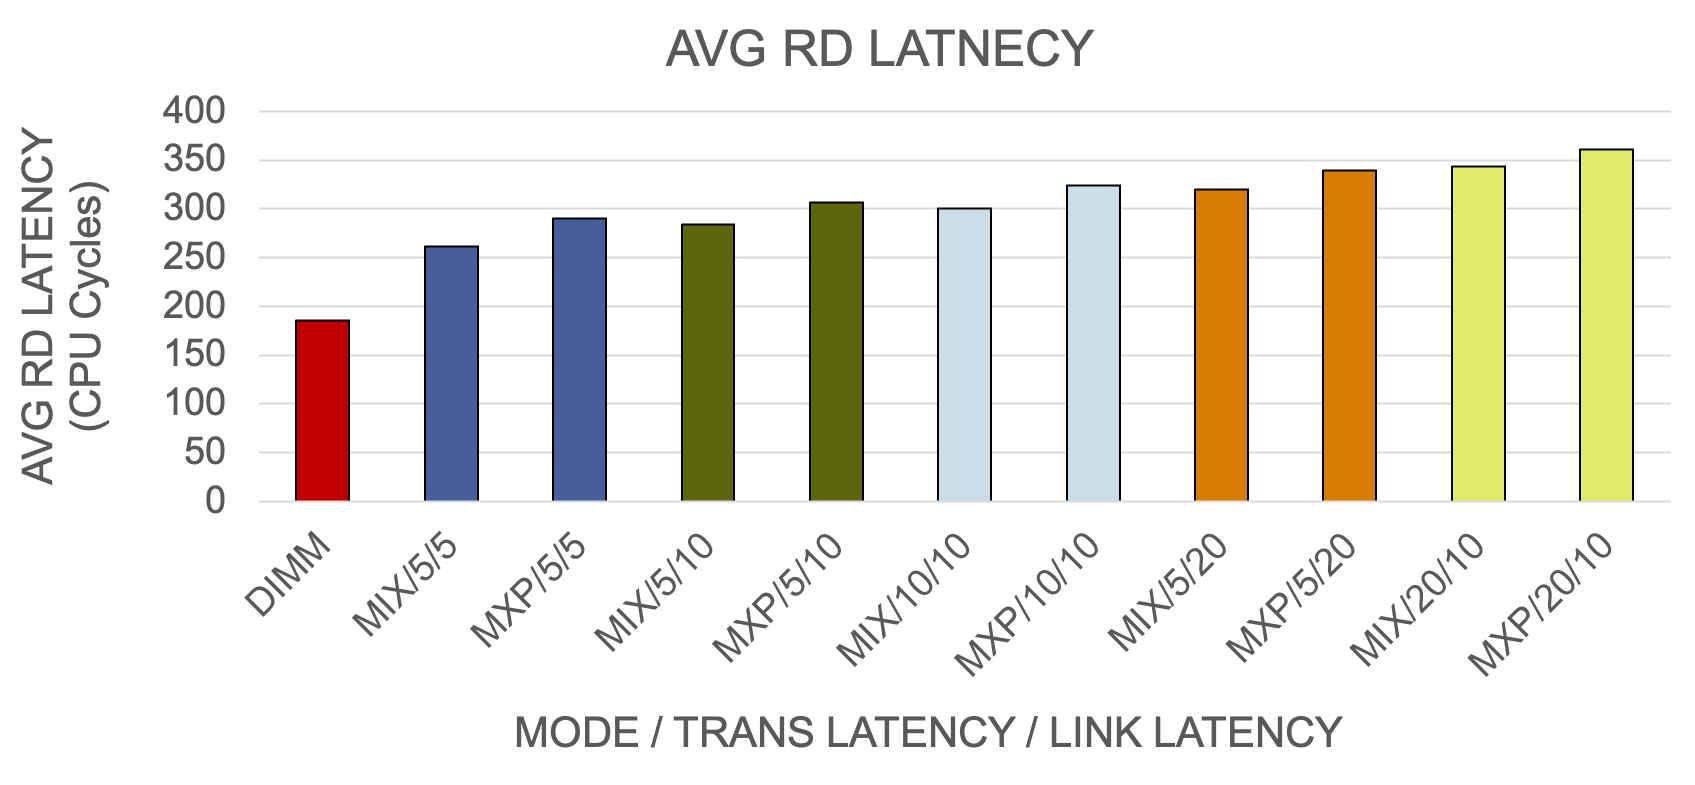
\includegraphics[width=\textwidth]{figures/avg rd latency.png}
  \caption{Average CXL type 3 device read latency of MIX and MXP subject to transaction layer, data link layer latency.}
  \label{fig:avg-rd-latency}
\end{figure}

On Figure \ref{fig:avg-rd-latency}, as sum of transaction layer latency and data link layer latency increases, the average read latency also increases. Since there's no commercially available CXL type 3 device yet, it's very difficult to exactly verify the correctness of this simulator. It's possible to compare the result with published papers like \cite{first-generation}, but exact validation is not easy. This result might be useful to verify against real CXL type 3 device and determine the latency in each layer. Also graph shows that always MIX shows slightly low latency than MXP with same configuration. MIX allocates half of pages to local DRAM, while MXP allocates all the pages to CXL type 3 device. Thus MIX has lower memory pressure on CXL type 3 device. This may lead to reduction in memory internal latency such as queuing delay.

Figure \ref{fig:dimm-rd-latency} shows local DRAM read latency of DIMM and MIX for 8 workloads. In case of MIX, the bar name follows the rule of Figure \ref{fig:avg-rd-latency}. The metric of read latency is CPU cycle. 

\begin{figure}[ht]
  \centering
  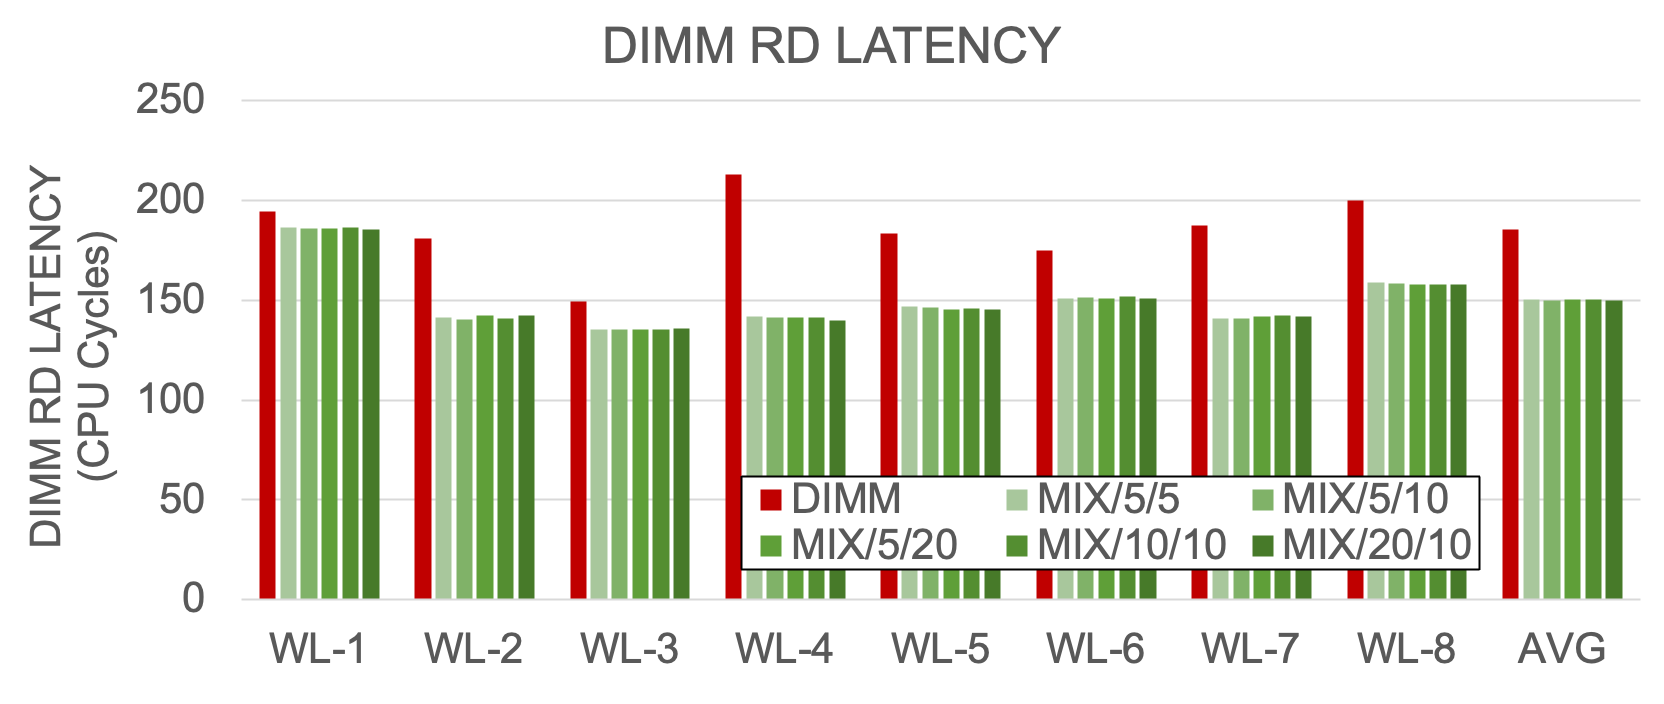
\includegraphics[width=\textwidth]{figures/dimm rd latency.png}
  \caption{Local DRAM read latency of DIMM and MIX.}
  \label{fig:dimm-rd-latency}
\end{figure}

Figure \ref{fig:dimm-rd-latency} shows local DRAM access latency of DIMM and MIX. On average, DIMM's local DRAM read latency is 185.43 cycles while MIX's local DRAM read latency is 150.2 cycles. As mentioned about Figure \ref{fig:avg-rd-latency}, MIX allocates half of pages to CXL type 3 device and leftover pages to local DRAM. In contrast, all the pages are allocated to local DRAM in DIMM. Thus DIMM has higher pressure on local DRAM than MIX. This pressure may influence memory latency such as queuing delay. So DIMM shows higher latency than MIX. Between MIXs with different transaction layer, data link layer latency, there was no significant latency difference. This is natural, since transaction layer and data link layer latency are related to CXL type 3 device and have nothing to do with local DRAM. This result implies that by adopting CXL type 3 device, we can expand memory capacity and reduce local DRAM access latency at the same time. However, CXL type 3 device has significantly high access latency. Thus we should well distribute memory traffic to exploit both large memory capacity and shortened local DRAM latency.